\documentclass[11pt]{article}
\usepackage{graphicx} % Required for inserting images
\usepackage{amsmath}
\usepackage{amssymb}
\usepackage{blindtext}
\usepackage{geometry}
\geometry{
 a4paper,
 left=30mm,
 right=30mm,
 top=30mm,
 bottom=30mm
 }
\usepackage{indentfirst}
\usepackage{setspace}
\usepackage{kotex}
\hbadness=99999 


\begin{document}

\title{Simulated Annealing for Rounded Capacity Inequality}
\author{Sangil Han}
\date{February 2024}
\maketitle
\begin{spacing}{1.5}
\begin {abstract}
    Capacitated Vehicle Routing Problem is a well-known routing problem. By using it, we can solve many logistics problems. However, this problem is known as NP-hard so we use the the Branch-and-Cut algorithm. In Branch-and-Cut algorithm, we must get a violated Rounded Capacity Inequality(RCI) to cut. The exact RCI separation algorithm is also known as NP-hard. Therefore, we use a heuristic algorithm for RCI separation to get violated RCI in a reasonable time. The most well-known heuristic algorithm is CVRPSep, but it just finds violated RCI not considering the performance. To get the best violated RCI, we would like to use the Simulated Annealing(SA) algorithm. To improve the performance of SA, we also design a specific neighborhood solution searching method for RCI separation.
\end{abstract}

\thispagestyle{empty}

\newpage
\thispagestyle{empty}
\tableofcontents

\newpage
\setcounter{page}{1}
{\centering \section {Introduction} \subsection{Branch-and-Cut Algorithms for CVRP}}
Capacitated Vehicle Routing Problem(CVRP) is an optimization problem distributing goods from a central depot to multiple customers using a fixed number of vehicles while considering each vehicle's limited capacity. Naddef and Rinaldi(2002) defined CVRP as follows\cite{CVRP}. $V$ is a node-set containing $n+1$ nodes numbered $0,1,...,n$. The node $0$ corresponds to the depot, and the other nodes correspond to the n customers. $V_0$ is the set of customers, i.e., $V_0=V\texttt{\char`\\}{0}$. Each customer $i$ wants as much as $d_i$ and each edge $e$ has a positive cost $c_e$. Let $K$ be the fixed number of vehicles. Each vehicle has the same capacity $C$. $x_e$ is the number of times $e$ appears in the $K$-route $R$ which is the union of $K$ routes $R_1,\; R_2,\;...,\;R_K$. For a subset $F$ of edge set $E$, and for a vector $x\in	\mathbb{R} ^E$, $x(F)$ means $\sum_{e\in F}x_e$. For $S \subset V$, $\delta(S)$ means an edge-set of edges that one endpoint is in $\delta(S)$ and the other in $V\texttt{\char`\\}S$. The ILP of CVRP is given by:

\begin{align}
     min \sum_{e \in E} c_ex_e
\end{align}
\qquad\qquad\qquad\qquad\qquad\qquad subject to
\begin{align}
    &&&&&&& x(\delta(i))=2   &\forall i \in V_0\\
    &&&&&&& x(\delta(0))=2K \\
    &&&&&&& x(\delta(S))\geq2\left\lceil\frac{d(S)}{C}\right\rceil &\forall\emptyset\neq S\subseteq V_0\\
    &&&&&&& 0\le x_e\le1  &\forall e\in E \texttt{\char`\\}\delta(0) \\
    &&&&&&& 0\le x_e\le2 &\forall e\in \delta(0) \\
    &&&&&&& x_e\;integer &\forall e\in E
\end{align}
\\We must focus on (4), Rounded Capacity Inequality. The left-hand-side means the number of times the vehicles in the $K$-route cross between the set $S$ and $V\texttt{\char`\\}S$. The right-hand-side roughly means two times the number of vehicles needed to serve all customers in $S$.
\indent Because it's hard to solve ILP, we first do linear relaxation by dropping (7). The LP is still difficult because the size of (4) is exponential. We can use the cutting plane technique. The cutting plane algorithm is as follows. We remove (4) and get optimal solution $x^*$. If $x^*$ is feasible for ILP, it is an optimal solution for ILP. Otherwise, we must use a separation algorithm. It gives us one constraint in (4) violated by $x^*$ if exists. We can get an updated optimal solution after adding the constraint. Repeat it until getting the optimal solution for ILP or relaxation for ILP. If we get an optimal solution of relaxation of ILP, we must use the branch-and-bound algorithm to get the optimal solution of ILP.


{\centering\subsection {Exact Separation for Rounded Capacity Inequality}}
The exact separation algorithm for RCI can be represented by MILP. Fukasawa et al.,(2004) defined the exact RCI separation algorithm as follows\cite{RCI}. $\bar{x_{ij}}$ is fractional value. Define $y_i$ as a binary variable equal to $1\;\text{if}\; i\in S\subset V$ and $w_{ij}$ as a variable equal to $1$ if an edge $(i,j)\; \text{belongs to}\; \delta(S)$. For each value of $M$ in \{$0,...,\left\lceil\frac{d(V_0)}{C}\right\rceil-1$\}, we solve:
    
\begin{align}
     z=min \sum_{e \in E} \bar{x_{ij}}w_{ij}
\end{align}
\qquad\qquad\qquad\qquad\qquad\quad subject to
\begin{align}
    &&&&&&& w_{ij} \geq y_i - y_j &\forall \{i,j\}\in E\\
    &&&&&&& w_{ij} \geq y_j - y_i &\forall \{i,j\}\in E\\
    &&&&&&& \sum_{i\in V_0}d_iy_i \geq (M\cdot C)+1\\
    &&&&&&& y_0=0\\
    &&&&&&& y_i\in\{0,1\} &\forall i\in V_0\\
    &&&&&&& w_{ij} \geq 0 &\forall \{i,j\}\in E
\end{align}
\\
\indent If $z<2(M+1)$, then $y$ is the violated set. The MILP is known as NP-hard. Therefore, it's hard to use exact separation.

\newpage
{\centering\section{Simulated Annealing}\subsection{Overview of SA}}
To get the violated RCI in a reasonable time, we can use the Simulated Annealing algorithm. It is a well-known meta-heuristic algorithm. Thanks to an efficient Metropolis acceptance criterion, SA can escape from local minima. The pseudo-code of SA is as follows.
\begin{figure}[htb!]
    \centerline{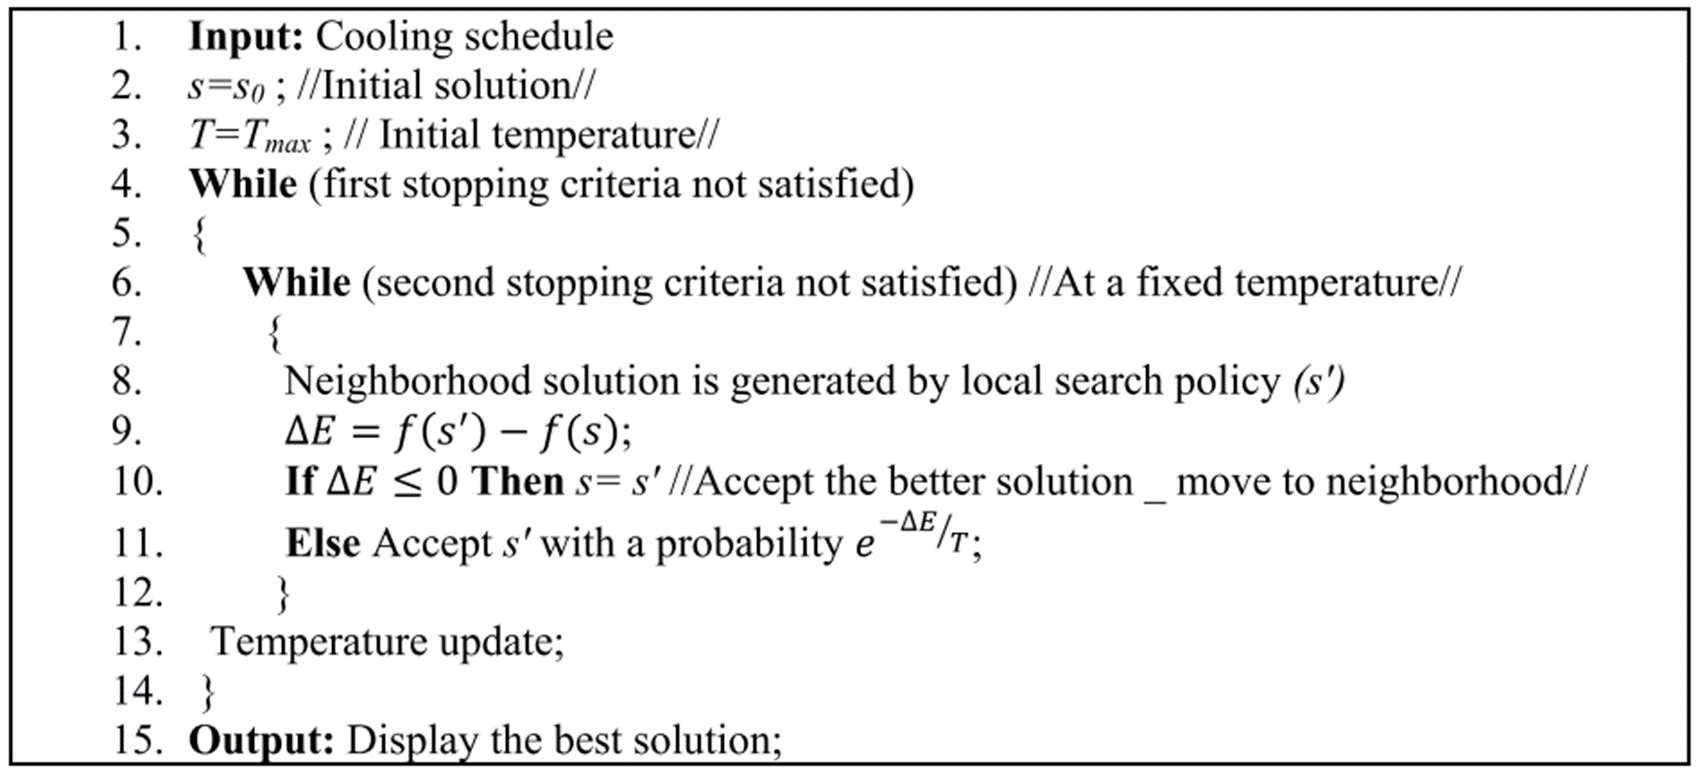
\includegraphics[width=15cm]{image1.png}}
    \caption{Pseudo code of SA}
\end{figure}
\\ 
\indent To perform SA, we need to set a cooling schedule, an initial solution, and how to get a neighborhood solution. The cooling schedule consists of initial temperature, temperature update function, stopping criterion, and length of Markov chain.


{\centering\subsection{Initial Temperature}}
When setting the initial temperature, we must consider the acceptance rate. It means the acceptance probability of the neighborhood solution for the initial solution. The higher the acceptance rate is, the better the performance of SA is. However, the number of iterations increases as the acceptance rate increases and it makes the longer runtime. The recommended value for acceptance rate is $0.8$.\\
\indent Delahye, Chaimatanan, and Mongeat(2019) find the acceptance rate and initial temperature as follows\cite{SA}. Let $m_1$ be the number of transitions that improves the objective function value, and $m_2$ be the number of the other transitions. Moreover, let $\bar{\Delta_f}^{(+)}$ be the average of the objective function value differences over all the not improved transitions. Then, the acceptance rate can be approximated by:
\begin{align}
    \chi(c) \simeq \frac{m_1+m_2\cdot e^{-(\frac{\bar{\Delta_f}^{(+)}}{c})}}{m_1+m_2}
\end{align}
which yields
\begin{align}
    c \simeq\frac{\bar{\Delta_f}^{(+)}}{ln(\frac{m_2}{m_2\cdot\chi(c)-m_1\cdot(1-\chi(c)})}
\end{align}
\indent If we set $m_1, m_2$ arbitrary, and $\chi(c)$ to $0.8$, we can get the initial temperature.


{\centering\subsection{Temperature Update Function}}
The temperature update function makes the temperature decrease. The most well-known and simple temperature update function is given by:
\begin{align}
     &&&&&&T_{k+1}=\alpha\cdot T_k  &&(0.8 \le\alpha\le0.99)
\end{align}


{\centering\subsection{Stopping Criterion}}
Stop criterion can be set using current temperature, run time, iteration number, etc. The general method is using the current temperature. If $T_k$ is closer to $0$, we can stop SA. The most well-known and simple stop criterion is given by:
\begin{align}
    T_k<0.01
\end{align}

{\centering\subsection{Length of Markov Chains}}
The length of Markov chains($L_k$) is a transition number at a fixed temperature. Because the neighborhood solution and Metropolis acceptance criterion are influenced only by the current solution, we can regard the transitions as a Markov chain. Delahye et al.,(2019) find $L_k$ as follows\cite{SA}. $L_k$ is related to the probability that a neighborhood solution can be visited. The average number of elements of set $S$ visited during $N$ iteration is given by:
\begin{align}
    |S|\cdot[1-e^{-\frac{N}{|S|}}]
\end{align}
for large $N$ and large $S$. Let $S_i$ be a neighborhood solution set for a given solution $i$. If no transition is accepted and if $N=|S_i|$, the probability that a neighborhood solution is visited is $1-e^{-1} \simeq \frac{2}{3}$. A good choice for $L_k$ is $|S_i|$.


{\centering\subsection{Initial Solution}}
To start SA, we need an initial feasible solution. In RCI, the feasible solution is a set that doesn't include a depot node. In the study, 4 different initial solutions, selecting customers randomly, including all customers, selecting one customer with the most degree, and a solution of CVRPSep are used. CVRPSep is a package that finds violated sets using other heuristic algorithms. 


{\centering\subsection{Neighborhood Solution}}
The most well-known method to get a neighborhood solution is $n$-flip. It is a method that chooses $n$ nodes randomly and changes the value of selected nodes. $n$-flip is easy to use when the solution consists of binary variables.\\
\indent Another method to get a neighborhood solution is a hamming ball operator. Let $k$ be the number of balls, and $m$ be the number of flips. The current solution is divided by $k$. At each ball, $m$ nodes are selected randomly and the value of nodes are changed.\\
\indent These two methods are general method. To get a better solution, a more specific method focused on RCI separation can be used. When $S$ is a node-set, the objective function to get good RCI is given by:
\begin{align}
    min\;f=x(\delta(S))-2\left\lceil\frac{d(S)}{C}\right\rceil
\end{align}
To decrease the objective function value, we must decrease $x(\delta(S))$ or increase $\left\lceil\frac{d(S)}{C}\right\rceil$. Assume that we use $n$-flip. The probability that $\left\lceil\frac{d(S)}{C}\right\rceil$ is changed is low because $n$ is a small value due to the neighborhood solution set size. If it is too large, $L_k$ is also a big value and the runtime can be too long. Therefore, it's hard to decrease $\left\lceil\frac{d(S)}{C}\right\rceil$. Let's see $x(\delta(S))$. If the node that isn't an endpoint of edge in $\delta(S)$ is selected, then $|\delta(S)|$ must be increased and $x(\delta(S))$ also be increased after a flip. However, if the node that is an endpoint of edge in $\delta(S)$ is selected, then $|\delta(S)|$ can be decreased and $x(\delta(S))$ also can be decreased after a flip. We can assume that it's better to select nodes that are an endpoint of edge in $\delta(S)$. Let's say this method to \textbf{$\boldsymbol{n}$-flip in $\boldsymbol{\delta(S)}$}. [Figure 2] is an example of $n$-flip in $\delta(S)$. The numbers that are written in the nodes are the demand of nodes. $x_e = 1$ for the line, $x_e = 0.5$ for the dotted line. The nodes that can be selected are red. 
\begin{figure}[htb!]
    \centerline{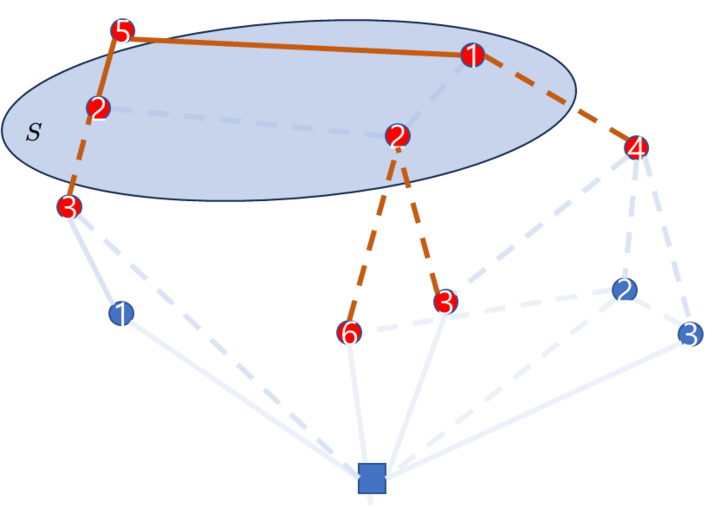
\includegraphics[width=7cm]{image2.png}}
    \caption{Example of $n$-flip in $\delta(S)$}
\end{figure}
\\ \\ \\ \\ \indent Moreover, let $k_i$ be the number of edges that are in $\delta(S)$ and whose one endpoint is node $i$. If $k_i$ is the same or bigger than $degree(i) - k_i$, $|\delta(S)|$ must not be increased after flipping for node $i$. It makes the probability that $x(\delta(S))$ is decreased higher. Let's say this method to \textbf{tight $\boldsymbol{n}$-flip in $\boldsymbol{\delta(S)}$}. [Figure 3] is an example of tight $n$-flip in $\delta(S)$. \\
\begin{figure}[htb!]
    \centerline{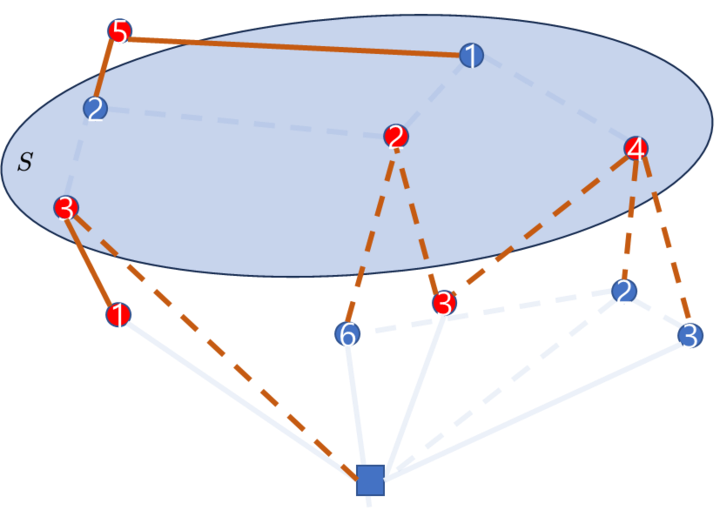
\includegraphics[width=7cm]{image3.png}}
    \caption{Example of tight $n$-flip in $\delta(S)$}
\end{figure}
\\ \indent Nodes that are an endpoint of edge in $\delta(S)$ can be divided into nodes in set $S$ and not in $S$. Let these two sets be $S_{in}$ and $S_{out}$. When we select nodes in $S_{out}$ to flip, we can select nodes that increase $\left\lceil\frac{d(S)}{C}\right\rceil$. We also can select nodes in $S_{in}$ that don't decrease $\left\lceil\frac{d(S)}{C}\right\rceil$. If we select nodes to flip in these nodes, the probability that the objective function value improves is high. Let's say this method to \textbf{$\boldsymbol{n}$-flip in $\boldsymbol{\delta(S)}$ considering demand}. [Figure 4] is an example of $n$-flip in $\delta(S)$ considering demand. Assume that the capacity is 10, select two nodes in $S_{out}$ and one node in $S_{in}$.\\
\begin{figure}[htb!]
    \centerline{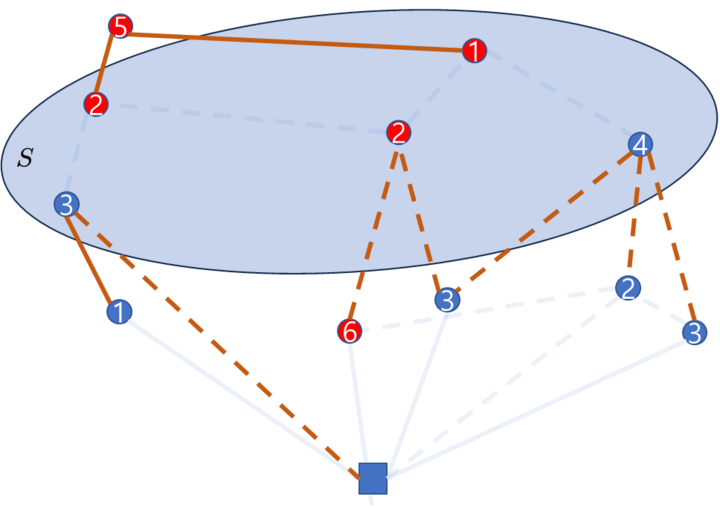
\includegraphics[width=7cm]{image4.png}}
    \caption{Example of $n$-flip in $\delta(S)$ considering demand}
\end{figure}
\\ \\ \\ \indent After a transition, we can improve the objective function value by adding the nodes that increase $\left\lceil\frac{d(S)}{C}\right\rceil$ to $S$. If $\left\lceil\frac{d(S)}{C}\right\rceil$ can be increased by just adding a node $i$, the objective function value must be the same or decrease because $x(\delta(i)) \le2$. If we need more than one node to increase $\left\lceil\frac{d(S)}{C}\right\rceil$, the objective function value can be increased after adding these nodes. 
However, if we allow to addition of only one node, the probability that the neighbor solution set is an empty set is high. Also, If we add more than one node, the solution that can be visited becomes diversified. When we set the number of added nodes as $k$, the node $i$ that can be selected must satisfy the condition, $\left\lceil\frac{d(S)+k\cdot d(i)}{C}\right\rceil > \left\lceil\frac{d(S)}{C}\right\rceil$. Let's say this method to \textbf{improvement method}. [Figure 5] is an example of the improvement method. Assume that the capacity is 10, and the number of added nodes is up to 2.
\begin{figure}[htb!]
    \centerline{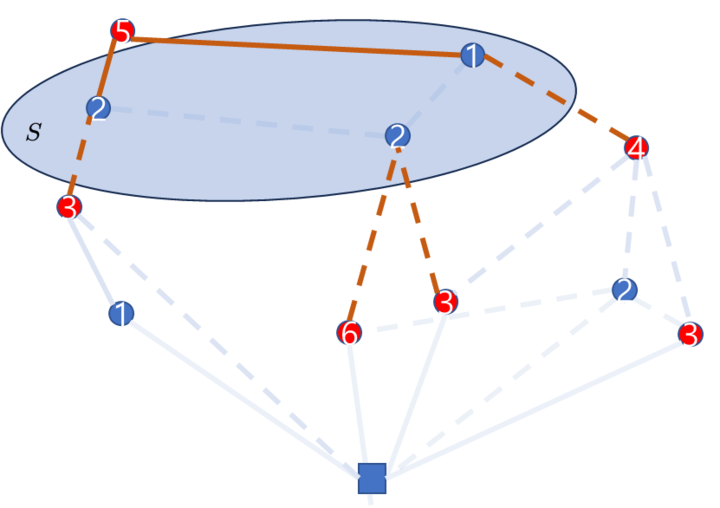
\includegraphics[width=7cm]{image5.png}}
    \caption{Example of improvement method}
\end{figure}
\\ \indent These methods can improve the objective function value after one transition. However, it doesn't guarantee that a better solution will be obtained after performing SA. 

\newpage
{\centering\section{Experiments}}
Using diverse initial solutions, neighborhood solution searching methods, and cooling schedule settings, we can perform SA with several settings. In the study, we used data about 50 nodes, 75 nodes, 100 nodes, and 200 nodes. Each data has different 100 graph data. The result can be evaluated by the gap and success rate. The gap is given by:
\begin{align}
    Avg\left(\frac{(-f_{\text{exact}})-(-f_{\text{SA}})}{(-f_{\text{exact}})}\right)
\end{align}
The success rate is given by:
\begin{align}
    \frac{\text{The number of success to find violated RCI}}{100}
\end{align}
\indent The gaps for several settings are as follows.

\begin{table}[!htb]
\resizebox{\textwidth}{!}{%
\begin{tabular}{|c|c|c|c|c|c|c|c|}
\hline
   & Initial Solution & Neighborhood Solution                            & $L_k$   & Gap\_50 & Gap\_75 & Gap\_100 & Gap\_200 \\ \hline
1  & all              & 1 flip                                    & $n$      & 55.7964 & 67.7561 & 72.1     & 90.9774  \\ \hline
2  & all              & 2 flip                                    & $4\cdot \binom n2$  & 11.4562 & 31.3429 & 39.9459  & 85.57    \\ \hline
3  & all              & 2 flip in $\delta(S)$                     & $4\cdot \binom {n_{in \; \delta(S)}}2$  & 32.5252 & 45.0197 & 50.0597  & 73.4208  \\ \hline
4  & one              & 2 flip                                    & $4\cdot \binom n2$   & 10.0987 & 24.7909 & 39.4349  & 67.5102  \\ \hline
5  & random           & 2 flip                                    & $4\cdot \binom n2$   & 10.8368 & 30.9756 & 37.6189  & 69.7466  \\ \hline
6  & CVRPSep          & 2 flip                                    & $4\cdot \binom n2$   & 6.6654  & 15.4478 & 20.9001  & 38.1849  \\ \hline
7  & CVRPSep          & 1 flip \& improvement                            & $4\cdot \binom n2$   & 9.1247  & 15.5408 & 15.178   & 17.5413  \\ \hline
8  & CVRPSep          & 2 flip \& improvement                            & $4\cdot \binom n2$   & 3.4905  & 7.8612  & 10.8351  & 16.8602  \\ \hline
9  & CVRPSep          & 2 flip in $\delta(S)$ \& improvement             & $4\cdot \binom n2$   & 0.9912  & 7.29    & 7.357    & 8.5917   \\ \hline
10 & CVRPSep & hamming ball operator\_3 \& improvement                                     & $(\frac{n}{3})^3$ & 3.0259 & 5.4181  & 11.6079 & 12.8734 \\ \hline
11 & CVRPSep          & hamming ball operator\_3 \& improvement                & $4\cdot \binom n2$   & 2.6748  & 7.6122  & 10.8091  & 21.2108  \\ \hline
12 & CVRPSep          & hamming ball operator\_4 \& improvement                & $4\cdot \binom n2$   & 2.6925  & 6.9041  & 7.6679   & 22.2573  \\ \hline
13 & CVRPSep          & hamming ball operator\_5 \& improvement                & $4\cdot \binom n2$   & 3.9527  & 9.0045  & 10.8749  & 22.4901  \\ \hline
14 & CVRPSep          & hamming ball operator\_2 \& improvement                & $4\cdot \binom n2$   & 3.4663  & 9.5997  & 11.6219  & 16.2258  \\ \hline
15 & CVRPSep          & 3 flip \& improvement                            & $4\cdot \binom n2$   & 3.1141  & 8.2442  & 8.6585   & 18.2919  \\ \hline
16 & CVRPSep          & 3 flip in $\delta(S)$ \& improvement               & $4\cdot \binom n2$   & 0.2748  & 4.3907  & 6.2751   & 15.9961  \\ \hline
17 & CVRPSep          & 3 flip in $\delta(S)$ considering demand \& improvement & $4\cdot \binom n2$   & 7.1066  & -       & -        & -        \\ \hline
18 & CVRPSep          & 2 flip in $\delta(S)$ considering demand \& improvement & $4\cdot \binom n2$   & 8.5847  & -       & 19.8768  & -        \\ \hline
19 & CVRPSep & 2 flip in $\delta(S)$ \& 2 flip in $\delta(S)$ considering demand \& improvement & $4\cdot \binom n2$                     & -      & 10.2669 & -       & -       \\ \hline
20 & CVRPSep & 2 flip in $\delta(S)$ considering demand \& improvement(accept only improved)                         & $4\cdot \binom n2$                     & 0.4815 & 4.0245  & 8.2993  & 11.605  \\ \hline
21 & CVRPSep          & 2 flip in $\delta(S)$ \& improvement(upto 1 node)       & $4\cdot \binom n2$   & 0.2533  & -       & 10.4175  & 29.0582  \\ \hline
22 & CVRPSep          & 2 flip in $\delta(S)$ \& improvement(upto 3 nodes)       & $4\cdot \binom n2$   & -       & -       & 11.6856  & -        \\ \hline
23 & CVRPSep & 2 flip in $\delta(S)$ \& 2 flip in $\delta(S)$ \& improvement               & $4\cdot \binom n2$                     & 0.1266 & 4.3646  & 6.6659  & 35.2763 \\ \hline
24 & CVRPSep          & tight 2 flip in $\delta(S)$ \& improvement       & $4\cdot \binom n2$   & -       & -       & 26.8237  & -        \\ \hline
\end{tabular}%
}
\caption{Gap between the result of SA and the exact RCI separation algorithm}
\label{tab:my-table}
\end{table}
\noindent The cooling schedule except for $L_k$ is the same. $\alpha = 0.95$. $L_k$ is originally the cardinality of the neighborhood solution set. However, to compare the performance of the searching methods, we also set $L_k$ to $4\cdot \binom n2$.   If two neighborhood solutions except for the improvement method that is case 19 and 23 are used, the second neighborhood solution is accepted only when it is an improved solution. Because some settings(case17, 18, 20, 21, 22, and 24) didn't show good value for some data, we don't perform SA with the setting for the other data. The default number of added nodes in the improvement method is 2. [Table 1] shows that the best initial solution is CVRPSEP, and the best searching method is $n$-flip in $\delta(S)$ except for $n=1$. When the improvement method with the default setting or accept-only-improved setting is added, the performance is much better.\\
\indent The success rates for several settings are as follows.
\begin{table}[!htb]
\resizebox{\textwidth}{!}{%
\begin{tabular}{|c|c|c|c|c|c|c|c|}
\hline
   & Initial Solution & Neighborhood Solution                            & $L_k$   & Success rate\_50 & Success rate\_75 & Success rate\_100 & Success rate\_200 \\ \hline
1  & all              & 1 flip                                    & $n$      &0.83  &0.66  & 0.75     &0.59   \\ \hline
2  & all              & 2 flip                                    & $4\cdot \binom n2$  &0.99  & 0.91 & 0.81  & 0.52    \\ \hline
3  & all              & 2 flip in $\delta(S)$                     & $4\cdot \binom {n_{in \; \delta(S)}}2$  &0.85  & 0.75 & 0.75  & 0.45  \\ \hline
4  & one              & 2 flip                                    & $4\cdot \binom n2$   &0.99  & 0.87 & 0.79  & 0.52  \\ \hline
5  & random           & 2 flip                                    & $4\cdot \binom n2$   & 0.97 & 0.83  &  0.82 & 0.49  \\ \hline
6  & CVRPSep          & 2 flip                                    & $4\cdot \binom n2$   & 0.98  & 0.9 & 0.89  & 0.85  \\ \hline
7  & CVRPSep          & 1 flip \& improvement                            & $4\cdot \binom n2$  &0.99  &0.94 &0.89   &0.93   \\ \hline
8  & CVRPSep          & 2 flip \& improvement                            & $4\cdot \binom n2$   &0.99  & 0.95& 0.93  &  0.93 \\ \hline
9  & CVRPSep          & 2 flip in $\delta(S)$ \& improvement             & $4\cdot \binom n2$   & 1 & 0.95&  0.95 &  0.98 \\ \hline
10 & CVRPSep & hamming ball operator\_3 \& improvement                                     & $(\frac{n}{3})^3$ &0.98  &0.97 & 0.91  &0.93   \\ \hline
11 & CVRPSep          & hamming ball operator\_3 \& improvement                & $4\cdot \binom n2$   &0.99  &0.96 &0.92   &0.89   \\ \hline
12 & CVRPSep          & hamming ball operator\_4 \& improvement                & $4\cdot \binom n2$   &1  &0.95 &0.96   & 0.88  \\ \hline
13 & CVRPSep          & hamming ball operator\_5 \& improvement                & $4\cdot \binom n2$   &0.99  &0.96 &0.92   & 0.9  \\ \hline
14 & CVRPSep          & hamming ball operator\_2 \& improvement                & $4\cdot \binom n2$   &0.99  &0.94 &0.93   &0.92   \\ \hline
15 & CVRPSep          & 3 flip \& improvement                            & $4\cdot \binom n2$   &0.99  & 0.95& 0.94  & 0.9  \\ \hline
16 & CVRPSep          & 3 flip in $\delta(S)$ \& improvement               & $4\cdot \binom n2$   &1  &0.96 & 0.95  & 0.9  \\ \hline
17 & CVRPSep          & 3 flip in $\delta(S)$ considering demand \& improvement & $4\cdot \binom n2$  &0.99  &- &-   &-   \\ \hline
18 & CVRPSep          & 2 flip in $\delta(S)$ considering demand \& improvement & $4\cdot \binom n2$   &0.98  &- &0.88   &-   \\ \hline
19 & CVRPSep & 2 flip in $\delta(S)$ \& 2 flip in $\delta(S)$ considering demand \& improvement & $4\cdot \binom n2$   &-  &0.94 &-   &-   \\ \hline
20 & CVRPSep & 2 flip in $\delta(S)$ considering demand \& improvement(accept only improved)                         & $4\cdot \binom n2$ &1  &0.97 &0.94   &0.95   \\ \hline
21 & CVRPSep          & 2 flip in $\delta(S)$ \& improvement(upto 1 node)       & $4\cdot \binom n2$  &1  &- & 0.94  &0.85   \\ \hline
22 & CVRPSep          & 2 flip in $\delta(S)$ \& improvement(upto 3 nodes)       & $4\cdot \binom n2$  &- &- &0.92   &-   \\ \hline
23 & CVRPSep & 2 flip in $\delta(S)$ \& 2 flip in $\delta(S)$ \& improvement               & $4\cdot \binom n2$  &1  &0.96 &0.95   &0.76   \\ \hline
24 & CVRPSep          & tight 2 flip in $\delta(S)$ \& improvement       & $4\cdot \binom n2$  &-  &- &0.85   &-   \\ \hline
\end{tabular}%
}
\caption{Success rate for the result of SA}
\end{table}

[Table 2] also shows that the best initial solution is CVRPSep and $n$-flip, $n$-flip in $\delta(S)$, and hamming ball operator with default or accept-only-improved improvement method are similar good searching methods. However, The success rate for 200 nodes data is especially high when the searching method is $2$-flip in $\delta(S)$.\\
\indent The average runtimes for several settings are as follow. The unit of runtime is sec.
\begin{table}[!htb]
\resizebox{\textwidth}{!}{%
\begin{tabular}{|c|c|c|c|c|c|c|c|}
\hline
   & Initial Solution & Neighborhood Solution                            & $L_k$   & Runtime\_50 &Runtime\_75 &Runtime\_100 &Runtime\_200 \\ \hline
1  & all              & 1 flip                                    & $n$      &0.009  &0.011  &0.014   &0.023  \\ \hline
2  & all              & 2 flip                                    & $4\cdot \binom n2$  &0.5  &1.2  &2.25   &9.42     \\ \hline
3  & all              & 2 flip in $\delta(S)$                     & $4\cdot \binom {n_{in \; \delta(S)}}2$  &0.17  &0.8  &1.8   &8.7   \\ \hline
4  & one              & 2 flip                                    & $4\cdot \binom n2$   &0.47  &1.1  &2   &8.7   \\ \hline
5  & random           & 2 flip                                    & $4\cdot \binom n2$   &0.36  &0.9  &1.5   &6.5   \\ \hline
6  & CVRPSep          & 2 flip                                    & $4\cdot \binom n2$   &0.5  &1.1  &2.1   &8.6   \\ \hline
7  & CVRPSep          & 1 flip \& improvement                            & $4\cdot \binom n2$  &0.8  &1.9  &3.4   &14.3   \\ \hline
8  & CVRPSep          & 2 flip \& improvement                            & $4\cdot \binom n2$   &0.8  &2  &3.7   &15.4  \\ \hline
9  & CVRPSep          & 2 flip in $\delta(S)$ \& improvement             & $4\cdot \binom n2$   &1.2  &3.3  &6.3   &30.6  \\ \hline
10 & CVRPSep & hamming ball operator\_3 \& improvement                                     & $(\frac{n}{3})^3$ &1.1  &4  &9   &73.2    \\ \hline
11 & CVRPSep          & hamming ball operator\_3 \& improvement                & $4\cdot \binom n2$   &1  &2.4  &4.6   &18.7    \\ \hline
12 & CVRPSep          & hamming ball operator\_4 \& improvement                & $4\cdot \binom n2$   &1.2  &3  &5.5  &23.1    \\ \hline
13 & CVRPSep          & hamming ball operator\_5 \& improvement                & $4\cdot \binom n2$   &1.4  &3.4  &6.4   &25.7   \\ \hline
14 & CVRPSep          & hamming ball operator\_2 \& improvement                & $4\cdot \binom n2$   &0.8  &2  &3.8   &15.5    \\ \hline
15 & CVRPSep          & 3 flip \& improvement                            & $4\cdot \binom n2$   &1.1  &2.8  &5   &22   \\ \hline
16 & CVRPSep          & 3 flip in $\delta(S)$ \& improvement               & $4\cdot \binom n2$   &1.5  &4.2  &8.3   &43.2   \\ \hline
17 & CVRPSep          & 3 flip in $\delta(S)$ considering demand \& improvement & $4\cdot \binom n2$  &1.8  &- &-   &-   \\ \hline
18 & CVRPSep          & 2 flip in $\delta(S)$ considering demand \& improvement & $4\cdot \binom n2$   &1.6  &- &7.6   &-   \\ \hline
19 & CVRPSep & 2 flip in $\delta(S)$ \& 2 flip in $\delta(S)$ considering demand \& improvement & $4\cdot \binom n2$   &-  &6.8 &-   &-   \\ \hline
20 & CVRPSep & 2 flip in $\delta(S)$ considering demand \& improvement(accept only improved)                         & $4\cdot \binom n2$ &4.8 &15.4 &30 &171.6   \\ \hline
21 & CVRPSep          & 2 flip in $\delta(S)$ \& improvement(upto 1 node)       & $4\cdot \binom n2$  &1.2  &-  &6.7   &35.6    \\ \hline
22 & CVRPSep          & 2 flip in $\delta(S)$ \& improvement(upto 3 nodes)       & $4\cdot \binom n2$  &-  &-  &6.7   &-    \\ \hline
23 & CVRPSep & 2 flip in $\delta(S)$ \& 2 flip in $\delta(S)$ \& improvement               & $4\cdot \binom n2$  &6  &18  &36   &198    \\ \hline
24 & CVRPSep          & tight 2 flip in $\delta(S)$ \& improvement       & $4\cdot \binom n2$  &-  &-  &5.5   &-   \\ \hline
\end{tabular}%
}
\caption{Rumtime for the result of SA}
\end{table}

\noindent [Table 3] shows that case 10, 20 and 23, the runtime is too long.

\indent Using CVRPSep, $n$-flip in $\delta(S)$, and default improvement, the performance is best. If SA for that setting iterates more, a better solution can be obtained. To make more iterations, we set the acceptance rate to 0.9, $\alpha = 0.98$, and the stopping criterion to $T_k\le0.001$. The result is as follows. To know how good the performance of SA is, we compared the result to the performance of CVRPSep. The results are shown in [Table 4], [Table 5], and [Table 6].
\begin{table}[!htb]
\resizebox{\textwidth}{!}{%
\begin{tabular}{|c|c|c|c|c|c|c|c|}
\hline
   & Initial Solution & Neighborhood Solution                            & $L_k$   & Gap\_50 & Gap\_75 & Gap\_100 & Gap\_200 \\ \hline
1  & CVRPSep              & 2 flip in $\delta(S)$ \& improvement       & $4\cdot \binom n2$      & 0.2983 & 5.1523 & 7.3447     & 5.4615  \\ \hline
2  & CVRPSep              & 3 flip in $\delta(S)$ \& improvement      & $4\cdot \binom n2$  & 0.2533 & 3.096 & 5.0226  & 8.1804   \\ \hline
3  & CVRPSep              &  -    & -  & 16.7526 & 30.4392 & 32.5385 & 43.4472  \\ \hline
\end{tabular}%
}
\caption{Gap for the best result of SA and CVRPSep}
\end{table}

\begin{table}[!htb]
\resizebox{\textwidth}{!}{%
\begin{tabular}{|c|c|c|c|c|c|c|c|}
\hline
   & Initial Solution & Neighborhood Solution                            & $L_k$   & Success rate\_50 & Success rate\_75 & Success rate\_100 & Success rate\_200 \\ \hline
1  & CVRPSep              & 2 flip in $\delta(S)$ \& improvement       & $4\cdot \binom n2$      &1 & 0.96 & 0.94 & 0.99 \\ \hline
2  & CVRPSep              & 3 flip in $\delta(S)$ \& improvement      & $4\cdot \binom n2$  & 1 & 0.97 & 0.95  & 0.97   \\ \hline
3  & CVRPSep              &  -    & -  & 0.97& 0.87 & 0.85 &0.73\\ \hline
\end{tabular}%
}
\caption{Success rate for the best result of SA and CVRPSep}
\end{table}

\begin{table}[!htb]
\resizebox{\textwidth}{!}{%
\begin{tabular}{|c|c|c|c|c|c|c|c|}
\hline
   & Initial Solution & Neighborhood Solution                            & $L_k$   & Runtime\_50 & Runtime\_75 & Runtime\_100 & Runtime\_200 \\ \hline
1  & CVRPSep              & 2 flip in $\delta(S)$ \& improvement       & $4\cdot \binom n2$      &5.2 & 14.1 & 26.6 & 141 \\ \hline
2  & CVRPSep              & 3 flip in $\delta(S)$ \& improvement      & $4\cdot \binom n2$  & 6.3 & 16.5 & 32.5  & 174   \\ \hline
\end{tabular}%
}
\caption{Runtime for the best result of SA}
\end{table}
Both the gap and success rate are improved a little. Compared to CVRPSep, both the gap and success rate are improved significantly. The runtimes are about 4 times longer.

\newpage
{\centering\section{Discussion}}
$n$-flip, $n$-flip in $\delta(S)$, tight $n$-flip in $\delta(S)$, and $n$-flip in $\delta(S)$ considering demand are more tight searching methods in order. That is, the probability that the solution after a transition is better than the current solution is higher in order. However, the performance is not better in order. Using $n$-flip in $\delta(S)$, the performance is the best. If tight $n$-flip in $\delta(S)$ or $n$-flip in $\delta(S)$ considering demand
is used, the cardinality of the neighborhood solution set is too small and it means it's hard to search diverse solutions. $n$-flip in $\delta(S)$ also makes a small cardinality of neighborhood solution set compared to $n$-flip, but it means only unnecessary solutions are excluded from searching using $n$-flip in $\delta(S)$. These results show it's important to design the appropriate solution-excluding method. Hamming ball operator also excludes some solutions, but it excludes some good solutions and shows worse performance.\\
\indent When the improvement method is used additionally, the performance is much better. The method makes SA search for more diverse solutions, particularly necessary solutions. $n$-flip in $\delta(S)$ only considers $x(\delta(S))$, but $2\cdot\left\lceil\frac{d(S)}{C}\right\rceil$ more influences to objective function value because $n$ is a small value.
To consider $2\cdot\left\lceil\frac{d(S)}{C}\right\rceil$, we designed other searching methods like tight $n$-flip in $\delta(S)$, and $n$-flip in $\delta(S)$. However, using these methods, the cardinality of the neighborhood solution set is too small and the performance is worse. On the contrary, the improvement method only searches for other solutions considering $2\cdot\left\lceil\frac{d(S)}{C}\right\rceil$ and it makes the performance much better.\\
\indent The performance of 1-flip in $\delta(S)$ is much worse than the other $n$-flip in $\delta(S)$ even with the same $L_k$. Using 1-flip in $\delta(S)$, the cardinality of the neighborhood solution set is $n$ and it's too small compared to $L_k$. Therefore, SA with 1-flip in $\delta(S)$ and $L_k = 4\cdot \binom n2$ may search the same neighborhood solution more compared to the other $n$-flip in $\delta(S)$. It makes it hard to search for a better solution.
\newpage
{\centering\section{Conclusion}}
The exact RCI separation algorithm is known as an NP-hard problem. To get the violated RCI in a reasonable time, we must use a heuristic algorithm. The most well-known method is using CVRPSep, but it doesn't consider the value of violation, i.e., $x(\delta(S)) - 2\cdot\left\lceil\frac{d(S)}{C}\right\rceil$. The value of violation determines the performance of the violated RCI. The higher the value is, the better the violated RCI. 
To get the best violated RCI, we use the Simulated Annealing algorithm. When the general method for neighborhood solution and arbitrary initial solution are used, the performance isn't good. However, If the output of CVRPSep is used for the initial solution and more specific neighborhood solution searching methods for RCI are used, the performance is improved much better. SA for RCI is better in performance than CVRPSep, but not in runtime. It's hard to use SA in the Branch-and-Cut algorithm because it needs many violated RCIs. SA can be used to make a comparative group for other heuristic algorithms about RCI separation, instead. The specific neighborhood solution searching methods also can be used to design other heuristic algorithms like the genetic algorithm. 

\newpage
\bibliographystyle{unsrt}
\bibliography{ref}



\end{spacing}
\end{document}
